\documentclass{ctexart}
\usepackage[utf8]{inputenc}
\usepackage{graphicx}
\usepackage{tikz}
\usetikzlibrary{shapes,arrows}


\title{图的模板类设计}
\author{陈科辉 Keiver Pabula}
\date{24 November,2022}
\begin{document}
\maketitle

\section{数据结构}
首先我所知道的数据结构有:树(二叉树,二叉搜索树,AVLTree,SplayTree),堆(二叉堆),图(有向图,无向图),数组,链表,栈(stack),散列表:对于数组是可以在内存中存储多个元素的结构,且存储是连续的,可以通过下标访问;栈是特殊的线性表,他仅能操作末端的数所以说是先进后出;队列也是一种现行表,但是它可以同时在先进先出的,从一端放入从另一端释;链表是物理存储单元上非连续的、非顺序的存储结构,每个元素包含两个结点,一个是存储元素的数据域,另一个是指向下一个结点地址的指针域;树也是一种数据结构,它由n个节点组成,有几层的关系,他的根节点在最上层,叶节点在其的下面,每个根只有一个父节点,但是一个父节点可以有多个字节点;Hash表是根据关键码和值 直接进行访问的数据结构,通过key和value来映射到集合中的一个位置;堆是特殊的数据结构与树类似,但是它是个完全二叉树且它的节点值永远要一直小于或一直大于它的父节点的值;图这个数据结构是由n个顶点加上连接两个顶点的边组成的图,而他的每个边都可以有个权值,图也有两个不同的边一个是有向的另一种是无向的,且他也有两种储存方式邻接表和邻接矩阵。

\section{设计思路}
首先我先做一个边类和顶点的类,分别做邻接表和邻接矩阵的存储方式;首先是对每个顶点我都给他用序号从0到n排序,然后初始化矩阵或列表,做一个空的矩阵和列表,初始值都为0,有连接他的值会变为他的权值。让用户输入数据u,v,w分别为他的头,尾巴和权值。通过print graph1和print graph2输出邻接矩阵和邻接矩阵。listVertexes输出各个顶点(为了方便读每个节点的前面加一个v),listEdges是把全部的边都列出来。

\section{测试结果}
以邻接矩阵的方式存储:
\begin{center}
  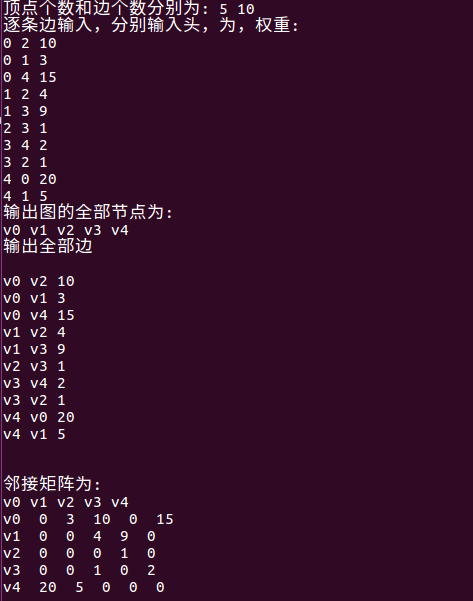
\includegraphics[scale=0.6]{ss2.png}
  \hspace{0.1in}
\end{center}
以邻接表的方式存储:
\begin{center}
  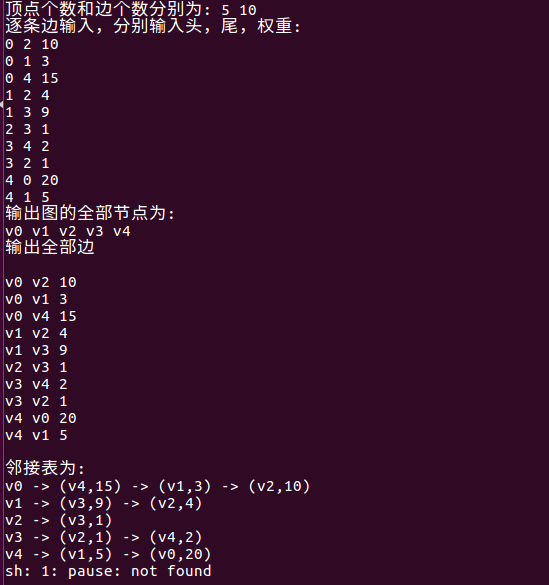
\includegraphics[scale=0.5]{ss3.png}
  \hspace{0.1in}
\end{center}


\end{document}
